\section{Search and Rescue}\label{sec:Search_and_Rescue}
When an emergency strikes, where people are stuck in a precarious place, unable to move, search and rescue operators must act fast to find the people in need and extract them. These missions occur in a variety of situations, but predominantly occur from natural disasters. It is said that the first 72 hours or less are the most critical for rescuing any remaining survivors \cite{SearchAndRescue:SAR_with_flying_robots}. However, without situational awareness of what has happened or a sense of where survivors could be, the operators are left helpless. Therefore, robots have been utilised to aid in the task of searching by creating a map of the environment.

\subsection{Natural disasters}
People around the world suffers every year from a various natural catastrophes such as the ones seen at the list below, causing harm and destruction to the environment, buildings, roads, which can result in people getting injured and in some cases casualties from the excessive weather conditions.
% Fortsætte med mere baggrundsviden om naturkatastrofer og hvilke kritiske episoder der kan opstå

\begin{itemize}\label{Natural_Disasters_List} % Evt. tilføje lidt beskrivende tekst til hver af natur fænomenerne 
    \item \textbf{Earthquakes:} When movement of the plates which the surface of earth constitute of, it affects the earth to shake and eventual the surface to rise or fall, in some occasions creating rift and breakage of the surface. These destructing shakes called earthquakes, can cause buildings to collapse, roads to crack and in less severe occasions things can fall apart which can lead to people getting trapped in affected buildings.  
    \item \textbf{Firestorms:} These instances occurs when the magnitude of a fire expands to such an extend that it creates a vacuum, pulling air against the fire. Meanwhile a pressure above the fire emerges, causing the fire to increase. In the worst scenario the fire will pull such an amount of air, that will form a fire whirl\footnote{Fire whirl is a tornado with fire in it}. Fires of these extends often happens in the wild from long periods of high temperature and drought, which ignites bushes and trees. However, they can also occur in cities from e.g. earthquakes. 
    \item \textbf{Floods:} Heavy rain can cause rivers, seas or lakes to overflow and rise above the ground level, causing the ground and sewers to fill, occasional leaving streets, basements and lower levels of building to be flooded. Potentially people are trapped and buildings will be harmed, leaving cities uninhabitable and sometimes casualties. 
    \item \textbf{Hurricanes:} Creation of what people experience as wind is raised from a low air pressure, which creates an air flow from an area with higher air pressure. When the low pressure drops even more, it can create a storm, these can increase in strength by the temperature of the surrounding air, resulting in the natural phenomena called hurricanes. These hurricanes can reach speeds up to 252 km/h, creating massive destruction on its way. \cite{SearchAndRescue:Hurricane_speeds}
    \item \textbf{Sand and dust storms:} These storms drags a vast amount of sand particles with them, which make it difficult for people to breath, see and navigate through the storm, potentially leading to traffic disasters and people getting stuck in sand, with no option of escaping. Sand and dust storms are formed in warm drought areas consisting primarily of sand. The high temperature in the area creates convection currents with speed up against 160 km/h, which brings much of the sand with the current, leading it far up into the atmosphere, increasing the spread of the sand. 
    \item \textbf{Tornadoes:} These destructive phenomenons are storms consisting of circular winds with speed up to 516 km/h and expands up to a width of several kilometres. A tornado is created from a cloud and reaching towards the ground right below it, lifting and moving objects of different size and causing buildings to collapse.  \cite{SearchAndRescue:largest_tornadoes}
    \item \textbf{Tsunamis:} When a earthquake happens on the bottom of the sea floor, it creates movement of the water, which is seen as waves travelling with a speed up to approximately 800km/h. As the movement of the water gets closer to the coast of land, the sea floor rises, causing the speed to be slower, but the waves to get larger.  \cite{SearchAndRescue:Tsunami_facts}
    \item \textbf{Volcanic eruptions:} Like how earthquakes occurs by movement of the earth plates, the same is established for volcanic eruptions. For these instances the plates move away from each other, alloying lava to float or sprout out of the opening rift. The hot lava will burn and melt almost anything in its path
\end{itemize}

% Summering af natur katastroferne, den generelle udfordring, samt hvilke ødelæggelser de forårsager

% Undersøgelse der viser omfanget af naturkatastrofer, samt deres udbredelse/lokation

\subsection{Building fires} % Her vil fokuseres mere på området af bygning brande startet af blandt andet naturkatastrofer. Som et fortsættene uddybning fra foregående sektion

% The cause of the fire. What happens? Introduction to how fires can be started from the natural disasters

% Escalation of the fire and expansion. How fast and wide does it spread? What is the reaction time for fire department 

% What is possible in the situation or what is not? Explanation of visibility, heat, air and additional conditions

% Damage and casualties from building fires

\subsection{Existing solutions}\label{subsec:ExistingSolutions}
In relation to search and rescue missions of building fires, several actions have been implemented and keep developing to encounter the following disasters. Fire brigades have for centuries been handling the tasks associated with building fires. These tasks includes securing the area against further accidents, extinguishing the fire and finding and rescuing people out of buildings. Various electronic systems is installed in buildings for observing for fire or smoke. These systems are identified from sensors alerting if smoke appears, to observation of the temperature in an area, enabling an alarm if its increases too vast. As this project aims to develop a robotic solutions able at assisting in search and rescue missions related to building fire, four different existing solutions will be presented to show the variety of current options available.  

\begin{figure}[H]
    \centering
    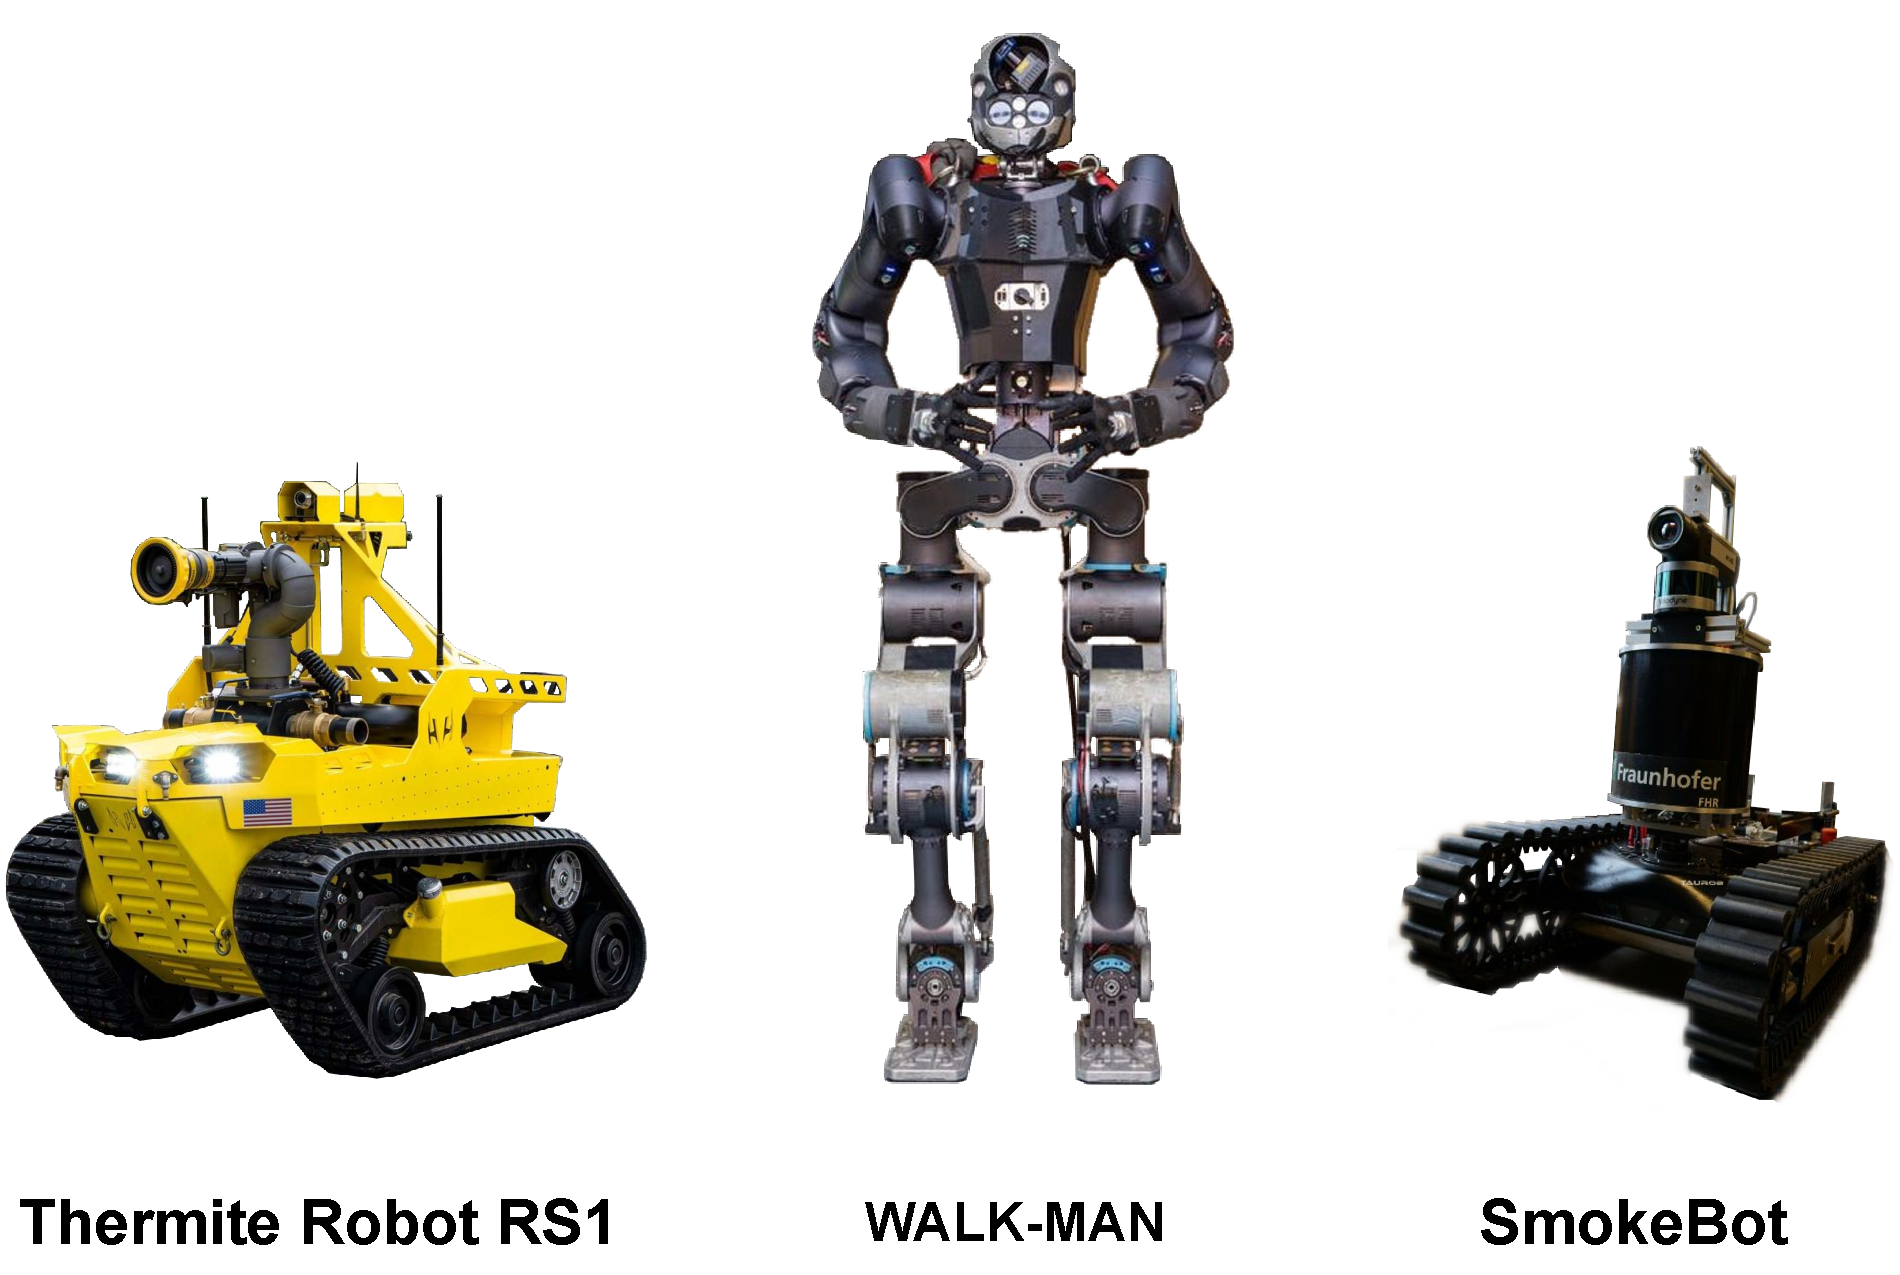
\includegraphics[width=0.7\textwidth]{figures/1Problem_analysis/Existing solutions.pdf}
    \caption{Three solutions aiming to aid in catastrophic situations of buildings in fire, reprinted from \cite{SearchAndRescue:Thermite_RS1}, \cite{SearchAndRescue:WALKMAN} and \cite{SearchAndRescue:SmokeBot}, respectively.}
    \label{fig:Existing_Solutions}
\end{figure}

\begin{description} 
    \item[Thermite Robot RS1] The robot manufactured by the company \textit{Howe X Howe} is equipped with tracks which makes it able to move in rough terrain with slopes up to 50\% increase and side slopes of maximum 35\% variance, making it capable of both climbing stairs and even push or overcome obstacles such as rubbles or collapsed objects. It is constructed to assist in building fires with a water flow of approx. 284 $m^3/h$ and a maximum pressure of 1.38 MPa. The Thermite RS1 is remote controlled and by a display offering the user to see high detailed videos with the possibility of infrared visibility. The robot is seen to the left in Figure \ref{fig:Existing_Solutions}. \cite{SearchAndRescue:Thermite_RS1}
    \item[WALK-MAN] Is a robot developed to help in cases of collapsed buildings after disasters caused by man or nature e.g. after a fire. The WALK-MAN is constructed with a powerful, but still robust balanced body able to both lift heavy objects or move over obstacles. The robot can operate autonomously or by tele-operation ensures it to maintain in function even in circumstances of poor communication possibilities. The WALK-MAN robot can be seen in the middle of Figure \ref{fig:Existing_Solutions} \cite{SearchAndRescue:WALK-MAN}
    \item[SmokeBot] Is a project by three universities and companies with interest of developing a product able to assist in search and rescue missions. The robot is specialised for navigation in situations with thick smoke, dust or fog, of which common robotic systems is not capable of mapping the environment. It navigates in these visually aggravated situations by a RGT-V unit\footnote{Abbreviation of Radar, gas sensor, thermal cameras and vision. Assembled into one sensing unit}, which makes the robot able to sense through visual obstacles and mapping the surfaces of e.g. a room in a building. The generated map can help the fire brigade to overview the situation of a building in fire before entering. An illustration of the solution can be seen to the right in Figure \ref{fig:Existing_Solutions} \cite{SearchAndRescue:SmokeBot}
    \item[Fire fighting drones] In general drones are used for different occasions in search and rescue operations, such as spraying water at buildings in fire, investigating areas to create a map or searching for people with need for help. Drones are very fast and manoeuvrable robots and depending on the size they can be able to enter almost any space. Especially flying drones will be capable of entering high floors, without going through the entire building from the ground floor. Drones can vary in size from the smallest called nano drones, measuring few centimetres to the largest drones with size similar of a helicopter. However, the majority of drones general used are mid-sized\footnote{width of the drone spanning from X m to X m} offering a good compromise between speed, weight capacity, price, steadiness and manoeuvrability. \cite{SearchAndRescue:Drone_size}
\end{description}

% Billede af droner kunne være fint

% Evt. opsummering af de eksisterenes fordele og ulemper i en tabel. 
% Tabel der fx. sammenligner: Fart, mobilitet, kostpris, vægt, dimensioner, funktionel tid og tilpasnings muligheder 
\begin{table}[H]
    \centering
    \resizebox{\textwidth}{!}{
    \begin{tabular}{?c|c|c|c|c|c?} \boldline
    \rowcolor{Gray!50}\textbf{Solution} & \textbf{Speed in m/s} & \textbf{Locomotion} & \textbf{Weight}  & \textbf{Runtime} & \textbf{Cost}\\\boldline
    Thermite Robot & ~2.68 & Tracks & & & \\ \hline
    WALK-MAN  &  & Legs and arms & &  & \\ \hline
    SmokeBot  &  & Tracks & &  &\\ \hline
    Drones  &  & Propellers & & & \\ \boldline
    \end{tabular}}
    \caption{.}
    \label{table:Existing_solutions}
\end{table}

% Delkonklusion om search and rescue
